\begin{figure}
    \centering
        \begin{subfigure}{.5\textwidth}
        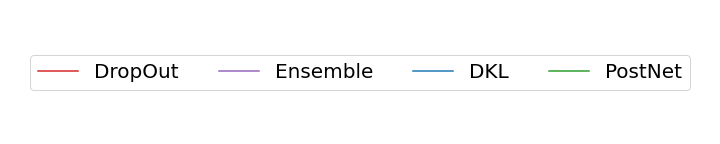
\includegraphics[width=\textwidth]{sections/011_icml2022/resources/legend.png}
    \end{subfigure}
    \vspace{-5mm}
    
    \begin{subfigure}{.245\textwidth}
        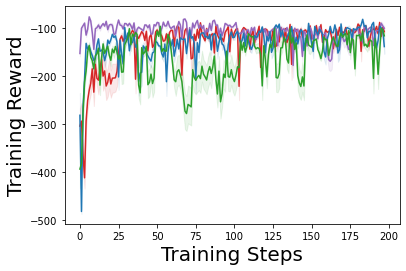
\includegraphics[width=\textwidth]{sections/011_icml2022/resources/acrobot-training_total_reward-training-model.png}
    \end{subfigure}
    \begin{subfigure}{.245\textwidth}
        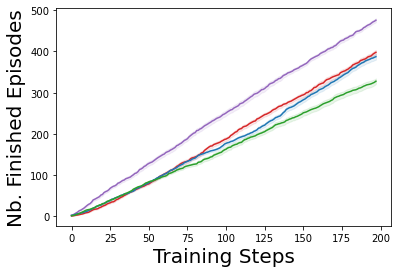
\includegraphics[width=\textwidth]{sections/011_icml2022/resources/acrobot-n_finished_training_episodes-training-model.png}  
    \end{subfigure}
    \begin{subfigure}{.245\textwidth}
        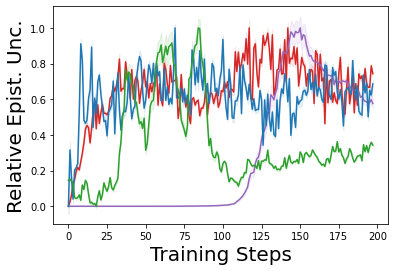
\includegraphics[width=\textwidth]{sections/011_icml2022/resources/acrobot-training_epistemic_uncertainty-training-model.png}
    \end{subfigure}
    \begin{subfigure}{.245\textwidth}
        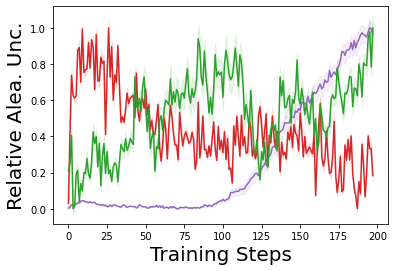
\includegraphics[width=\textwidth]{sections/011_icml2022/resources/acrobot-training_aleatoric_ucertainty-training-model.png}  
    \end{subfigure}
    \caption{Comparison of the training performance of the four uncertainty methods using epsilon-greedy strategies on Acrobot. Ideally, a uncertainty aware-model should achieve high reward with few samples and with a decreasing epistemic uncertainty.}
    \label{fig:model-training-performance-acrobot}
\end{figure}